\documentclass[17pt, a0paper, blockverticalspace=0.8cm, colspace=0.8cm]{tikzposter}

% Suppress some useless warnings
\usepackage{silence}
\WarningFilter{remreset}{The remreset package}
\WarningFilter{latex}{Font shape declaration has incorrect series value `mc'.}

% \usetheme{Default}
% \usetheme{Rays}
% \usetheme{Basic}
% \usetheme{Simple}
% \usetheme{Envelope}
% \usetheme{Wave}
\usetheme{Board}
% \usetheme{Autumn}
% \usetheme{Desert}

\usepackage[UKenglish]{babel}
\usepackage[style=alphabetic,maxbibnames=99]{biblatex}
\usepackage{amsmath}
\newcommand{\defeq}{\vcentcolon=}
\usepackage{mathtools}
\usepackage{amsthm}
\usepackage{csquotes}
\usepackage[inline]{enumitem}
\usepackage[capitalize,noabbrev]{cleveref}
\usepackage[final]{microtype}

% Fix me notes
\usepackage[draft]{fixme}
\usepackage{svg}
\fxusetheme{color}

\usepackage[charter]{mathdesign}
\usepackage[T1]{fontenc}

\title{Stochastic Gradient Hamiltonian Monte Carlo}
\author{Candidate Numbers: 1302365, 1059459, 1060482 and 1058141}
\institute{University of Oxford\vspace{-1.5em}}


% Bibliography
\addbibresource{../references.bib}

\begin{document}

	% \vspace*{-100em}
	\maketitle
	
		\begin{columns}

	%%% First column %%%%%%%%%%%%%%%%%%%%%%%%%%%%%%%%%%%%%%%%%%%%%%%%%%%%%
		\column{0.4}
		
	
	%%% Second column %%%%%%%%%%%%%%%%%%%%%%%%%%%%%%%%%%%%%%%%%%%%%%%%%%%%%
	   \column{0.6}
		

    	\end{columns}

	\begin{columns}

		%%% First column %%%%%%%%%%%%%%%%%%%%%%%%%%%%%%%%%%%%%%%%%%%%%%%%%%%%%
		\column{0.5}
		\block{Stochastic Gradient Hamiltonian Monte Carlo}{
		Hamiltonian Monte Carlo (HMC) provides us with a useful way to sample from a posterior distributions. To do this we require a potential function $U(\theta) \propto \log p(\theta | \mathcal{D})$, as well as means to compute the gradient. At each step HMC uses all the data available to it; evaluating $U(\theta)$ and computing $\nabla U(\theta)$ is computationally expensive for large datasets, rendering HMC almost useless. As such, this motivated the development of the Stochastic Gradient Hamiltonian Monte Carlo algorithm (SGHMC), which is introduced by the paper in question \cite{sghmc}. It uses randomly sampled mini-batches of data to produce noisy estimates of the gradient $\nabla \widetilde U(\theta)$, which gives SGHMC a significant speed-up compared to HMC. In this paper, Chen et al first introduce a Naive SGHMC algorithm, demonstrating the pitfalls of using noisy gradient estimates. They also introduce the full SGHMC algorithm that uses friction to overcome the need for a costly MH correction step. They further demonstrate the links between SGHMC and both Stochastic Gradient Descent (SGD) with momentum, and Stochastic Gradient Langevin Dynamics (SGLD). They then run experiments using SGHMC to empirically back up their theoretical claims and show that SGHMC is a candidate algorithm for scalable Bayesian inference. We implemented our own version of SGHMC along with some other algorithms and reproduced a number of Chen et al's experiments. The repository for our code can be found at \url{https://github.com/sacktock/SGHMC}.
	
		
	}
		\block{The Core Algorithms}{
		Below we introduce the major algorithms discussed in the paper. The first four algorithms are sampling algorithms - we sample parameters $\theta$ from the posterior distribution described by the model. We write here the transition steps that, upon iterating, gives us $\theta \sim p(\theta | \mathcal{D})$, where $\mathcal{D}$ is all the data available to us. $\tilde{\mathcal{D}}$ is a randomly sampled batch of this data. \\
		
\begin{minipage}[t]{0.43\linewidth}
	\innerblock{Hamiltonian Monte Carlo (HMC)}{
		$$\Delta \theta \leftarrow \epsilon M^{-1}r \qquad \Delta r \leftarrow - \epsilon \nabla U(\theta)$$
		where $$ \nabla U(\theta) \defeq - \sum_{x \in \mathcal{D}} \nabla \log p(x \mid \theta) -  \nabla \log p(\theta)$$}
\end{minipage}
\begin{minipage}[t]{0.57\linewidth}
\innerblock{Naive Stochastic Gradient Hamiltonian Monte Carlo (Naive SGHMC)}{$$\Delta \theta \leftarrow \epsilon M^{-1}r \qquad \Delta r \leftarrow - \epsilon \nabla \tilde{U}(\theta)$$
		where $$ \nabla \tilde{U}(\theta) \defeq - \frac{|\mathcal{D}|}{|{\tilde{\mathcal{D}}}|}\sum_{x \in \tilde{\mathcal{D}}} \nabla \log p(x \mid \theta) - \nabla \log p(\theta)$$}
\end{minipage}

\begin{minipage}[t]{0.7\linewidth}
		\innerblock{Stochastic Gradient Hamiltonian Monte Carlo (SGHMC)}{$$\Delta \theta \leftarrow \epsilon M^{-1}r \qquad \Delta r \leftarrow - \epsilon \nabla \tilde{U}(\theta) - \epsilon C M^{-1} r + \mathcal{N}(0,2 (C-\hat{B})\epsilon)$$
		where $$\nabla \tilde{U}(\theta) \defeq - \frac{|\mathcal{D}|}{|{\tilde{\mathcal{D}}}|}\sum_{x \in \tilde{\mathcal{D}}} \nabla \log p(x \mid \theta) - \nabla \log p(\theta)$$
		and $\hat{B}$ is an estimation of the noise covariance $B$ encapsulated by $\nabla \tilde{U}(\theta) = \nabla U(\theta) + \mathcal{N}(0,2 B\epsilon)$, and $C$ is a user-defined hyperparameter}
\end{minipage}
\begin{minipage}[t]{0.3\linewidth}
		\innerblock{Stochastic Gradient Langevin Dynamics (SGLD)}{$$\Delta \theta \leftarrow - \eta \nabla \widetilde U(\theta) + \mathcal{N}(0,B)$$
		
		where $B$ is the covariance of injected noise.\\}
	    \end{minipage}
		The final algorithm (SGD) is an optimization algorithm, the idea is it iteratively converges to the mode of the posterior distribution - giving us a point estimate, namely, a MAP estimate. \\

		\innerblock{Stochastic Gradient Descent (SGD)}{$$\Delta \theta \leftarrow  \alpha \Delta \theta - \eta \nabla \widetilde U(\theta)$$
		
		where $\alpha$ is a momentum hyperparameter. Standard SGD sets $\alpha=0$ } 
		
	}
	
	
\block{Bayesian Neural Networks for Classification}{Below we present the results of running our algorithms on MNIST and FashionMNIST. We ran each of the algorithms for 800 epochs with 50 warmup epochs and 100 warm up epochs for MNIST and FashionMNIST respectively. For all the experiments we subsampled the dataset with batch sizes of 500 images. For the posterior sampling algorithms (SGHMC and SGLD) we performed Bayesian averaging over all the sampled parameterisations of the BNN after warmup and report the test accuracy as described in Section II of \cite{hands-on-bnn}. For the optimization algorithms (SGD and SGD with momentum) we fixed the L2 regularization to $\lambda = 1.0$ and take the latest sample as point estimate and report the test accuracy.
			
            \begin{tikzfigure}[{\bf Left:} reproducing the MNIST classificiation experiment from \cite{sghmc} ; SGHMC ($\eta = 2.0\times 10^{-6}, \alpha=0.01, \texttt{resample\_n} =0$ ), SGLD ($\eta = 4.0\times 10^{-5}$), SGD ($\eta = 1.0\times 10^{-5}$), SGD with momentum ($\eta = 1.0\times 10^{-6}, \alpha=0.01$) ;\texttt{warmup\_epochs} $= 50$ {\bf Right:}  FashionMNIST classification experiment ; SGHMC ($\eta = 1.0\times 10^{-6}, \alpha=0.01, \texttt{resample\_n} =0$ ), SGLD ($\eta = 1.0\times 10^{-5}$), SGD ($\eta = 1.0\times 10^{-5}$), SGD with momentum ($\eta = 1.0\times 10^{-6}, \alpha=0.01$); \texttt{warmup\_epochs} $= 100$.]
            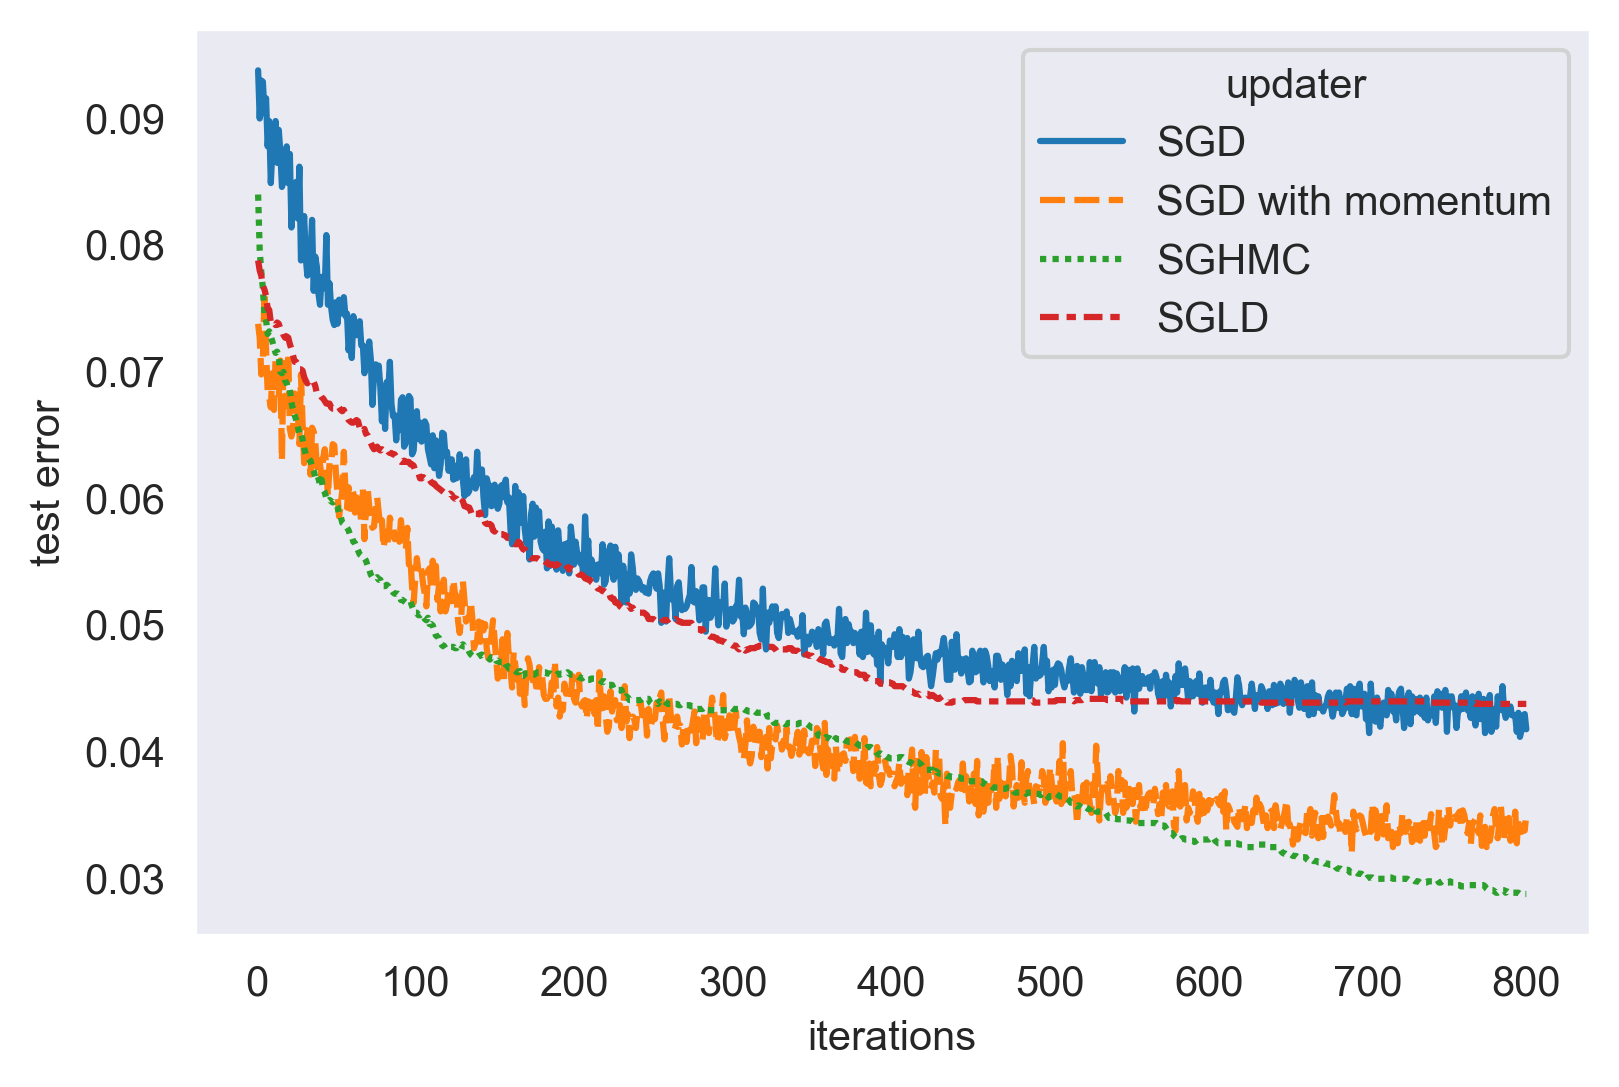
\includegraphics[width=150mm]{Images/MNIST.png}
            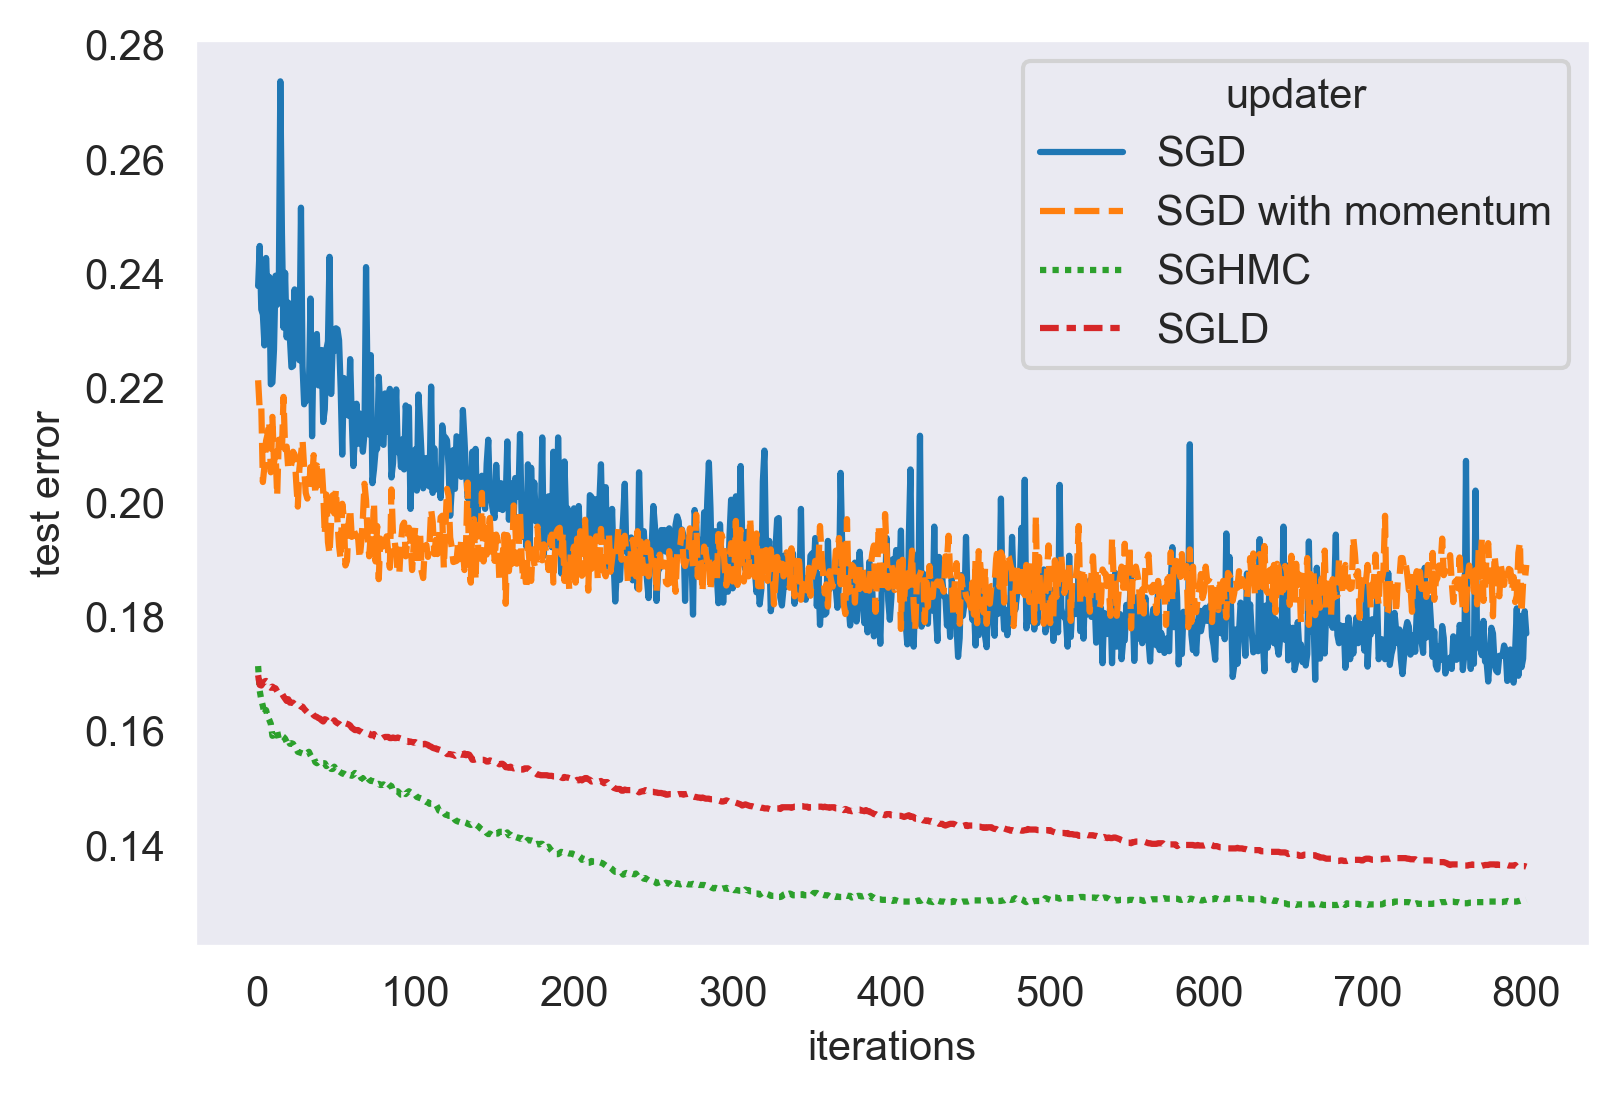
\includegraphics[width=150mm]{Images/fashion-mnist.png}
            \end{tikzfigure} 

        }
		\block{SGNUTS}{'Stochastic Gradient No U-Turn Sampler' (SGNUTS) is our novel algorithm based on the 'No U-Turn Sampler' (NUTS) produced in \cite{nuts}. NUTS removes the need for the user to pre-set the number of steps HMC performs before taking a sample. We produced SGNUTS to do the same for SGHMC. At its core, it works by repeatedly performing SGHMC steps either forward or backward in time until a 'U-turn' is seen. This is when a further step forwards in time would cause the latest sample in the trajectory to get closer to the earliest sample (or similarly for a step backwards in time). It reached accuracies of 0.94 on MNIST and 0.85 on FashionMNIST, which is similar to SGHMC (accuracies of 0.97 and 0.85 respectively). SGNUTS reaches the posterior faster than SGHMC, taking 28s to reach an accuracy of 0.87, compared to SGHMC taking 50s to reach 0.89. When at the posterior, SGNUTS takes longer than SGHMC to sample from it however.
		
		  \begin{tikzfigure}[SGNUTS Learning Curves on MNIST (left) and FashionMNIST (right)]
            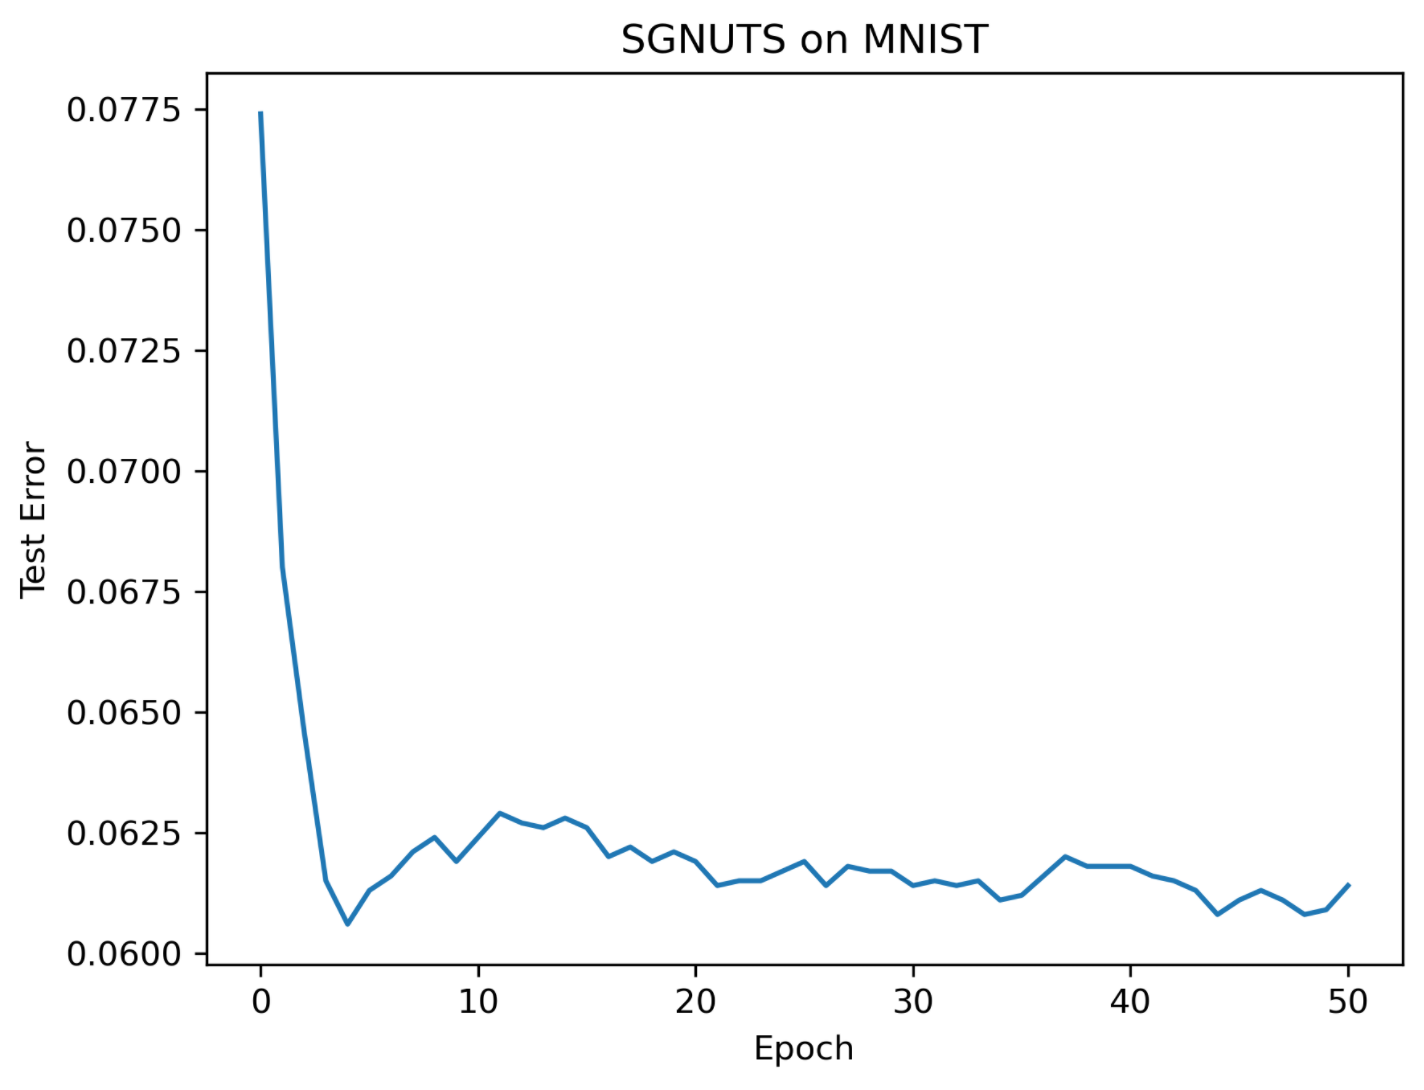
\includegraphics[width=120mm]{Images/SGNUTS_MNIST.png}
            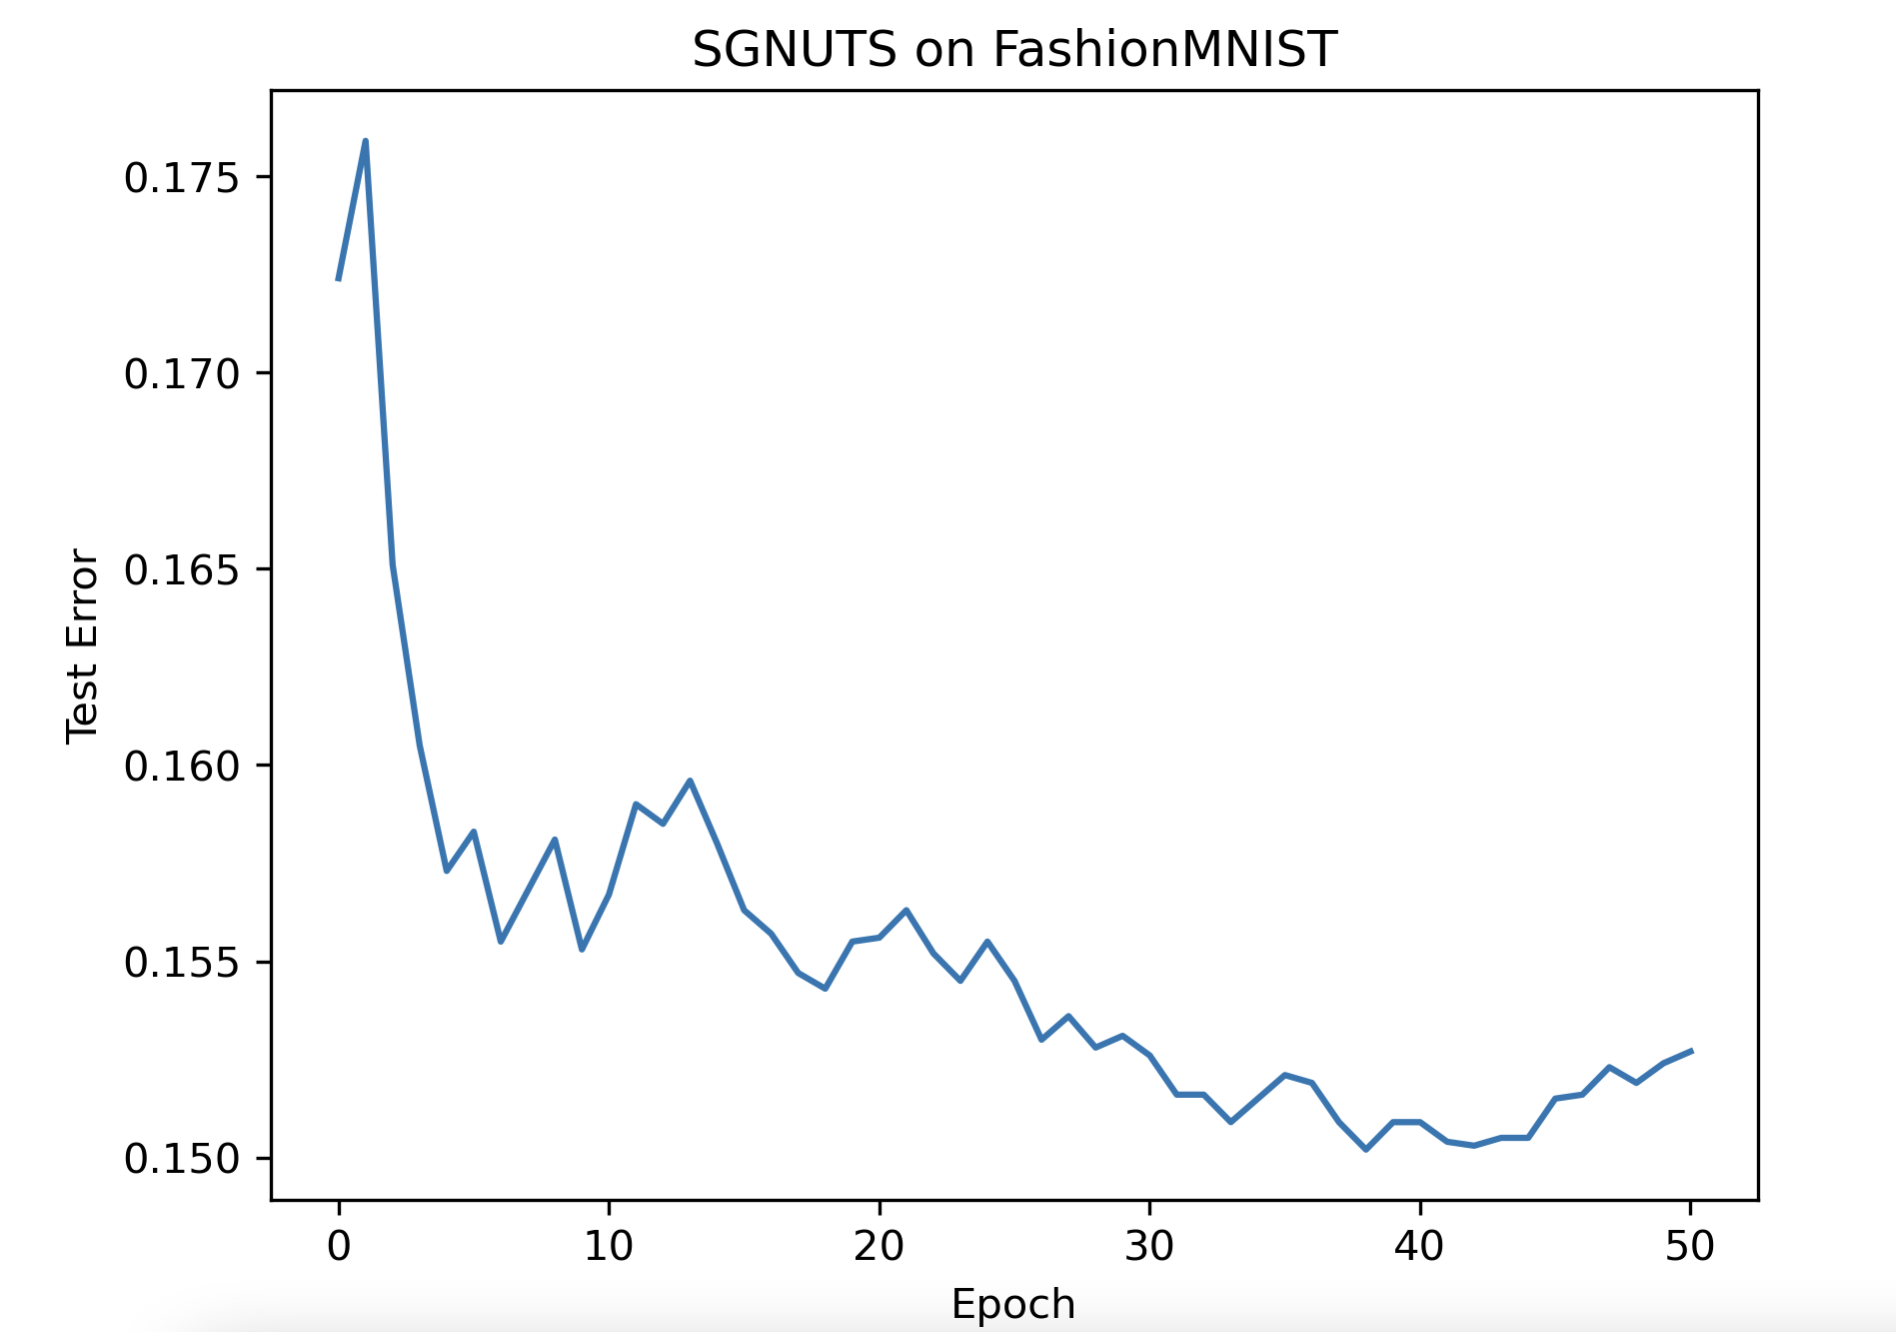
\includegraphics[width=120mm]{Images/SGNUTS_Fashion.png}
            \end{tikzfigure} }


			\block{Further Research}{
			\begin{itemize}
				\item Implementation of a hybrid SGNUTS and SGHMC algorithm - SGNUTS quickly reaches the posterior, however SGHMC is faster at sampling when at the posterior. We could investigate the power of using SGNUTS for the first few epochs or during warmup, followed by SGHMC.
			   \item Tuning the CNN used to classify CIFAR10. Currently we have shown that our implementation of SGHMC can start classifying CIFAR10, however we could acheive better accuracies with more time to investigate other architectures and do a more thorough hyperparameter search.
			   \item Further investigate methods of estimating the gradient noise $B$, as using empirical Fisher was computationally expensive for high dimensional models.
			   \item Compare more thoroughly our implementation of SGHMC to Variational Inference.
			\end{itemize}		}
		
		%%% Second column %%%%%%%%%%%%%%%%%%%%%%%%%%%%%%%%%%%%%%%%%%%%%%%%%%%%
		\column{0.5}
			\block{The Reproducibility Challenge and Extensions}{
	We reproduced the following experiments from the paper:
\begin{itemize}
    \item Sampling $\theta$ from the potential function $U(\theta) = -2\theta^2 + \theta^4$ with noise added to the gradient $\nabla \widetilde U(\theta)$, using the following algorithms: HMC (with and without MH correction), Naive SGHMC (with and without MH correction) and SGHMC.
    \item Using HMC to sample $(\theta,r)$ from the potential function $U(\theta) = \frac{1}{2}\theta^2$ with perfect gradients, and noisy gradients using $\mathcal{N}(0,4)$ as a proxy for the noise in $\tilde{U}(\theta)$.
    \item Comparing the autocorrelation times of SGHMC and SGLD.
    \item Classifying the MNIST dataset using SGHMC as well as with SGD, SGD with momentum, and SGLD.
\end{itemize} 
\begin{tikzfigure}[Some of the figures from \cite{sghmc} which we aimed to reproduce. {\bf Left:} using HMC to sample $(\theta,r)$. {\bf Center:} Samples from the potential function $U(\theta) = -2\theta^2 + \theta^4$. {\bf Right:} learning curves for MNIST classification]
            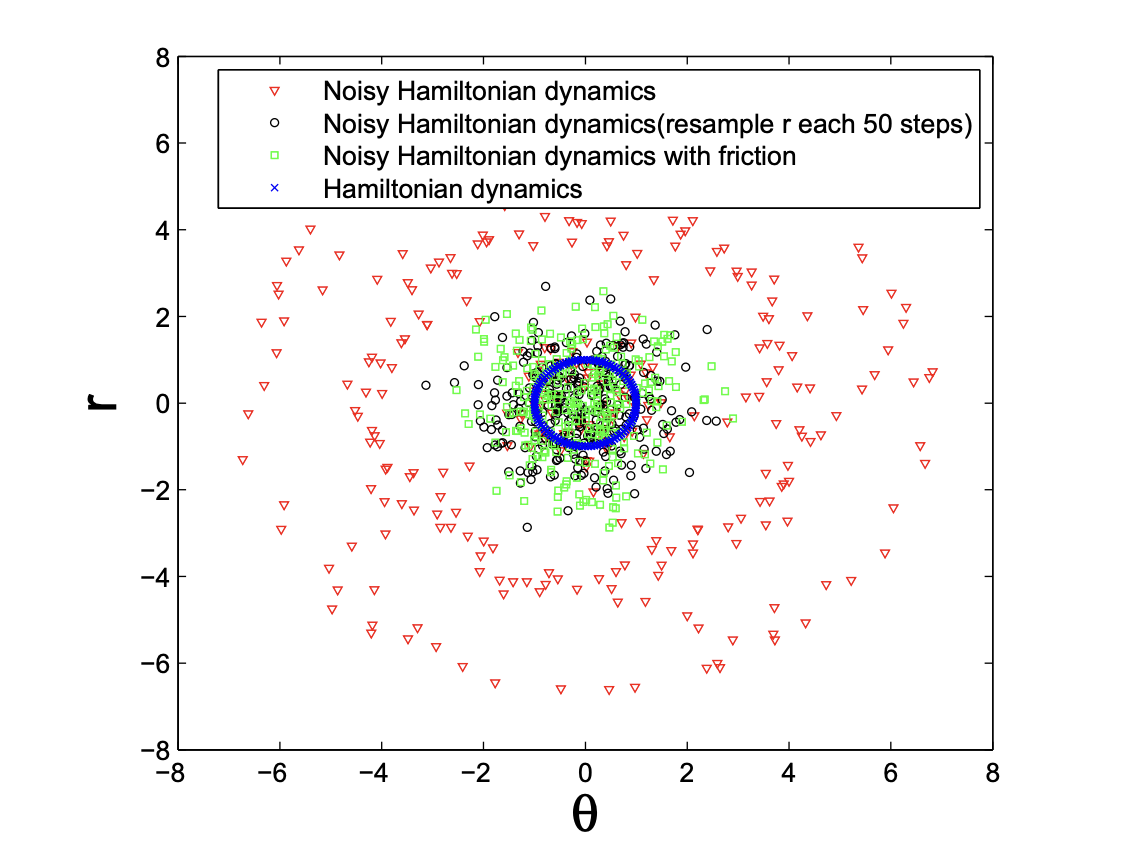
\includegraphics[width=100mm]{Images/reproduce1.png}
            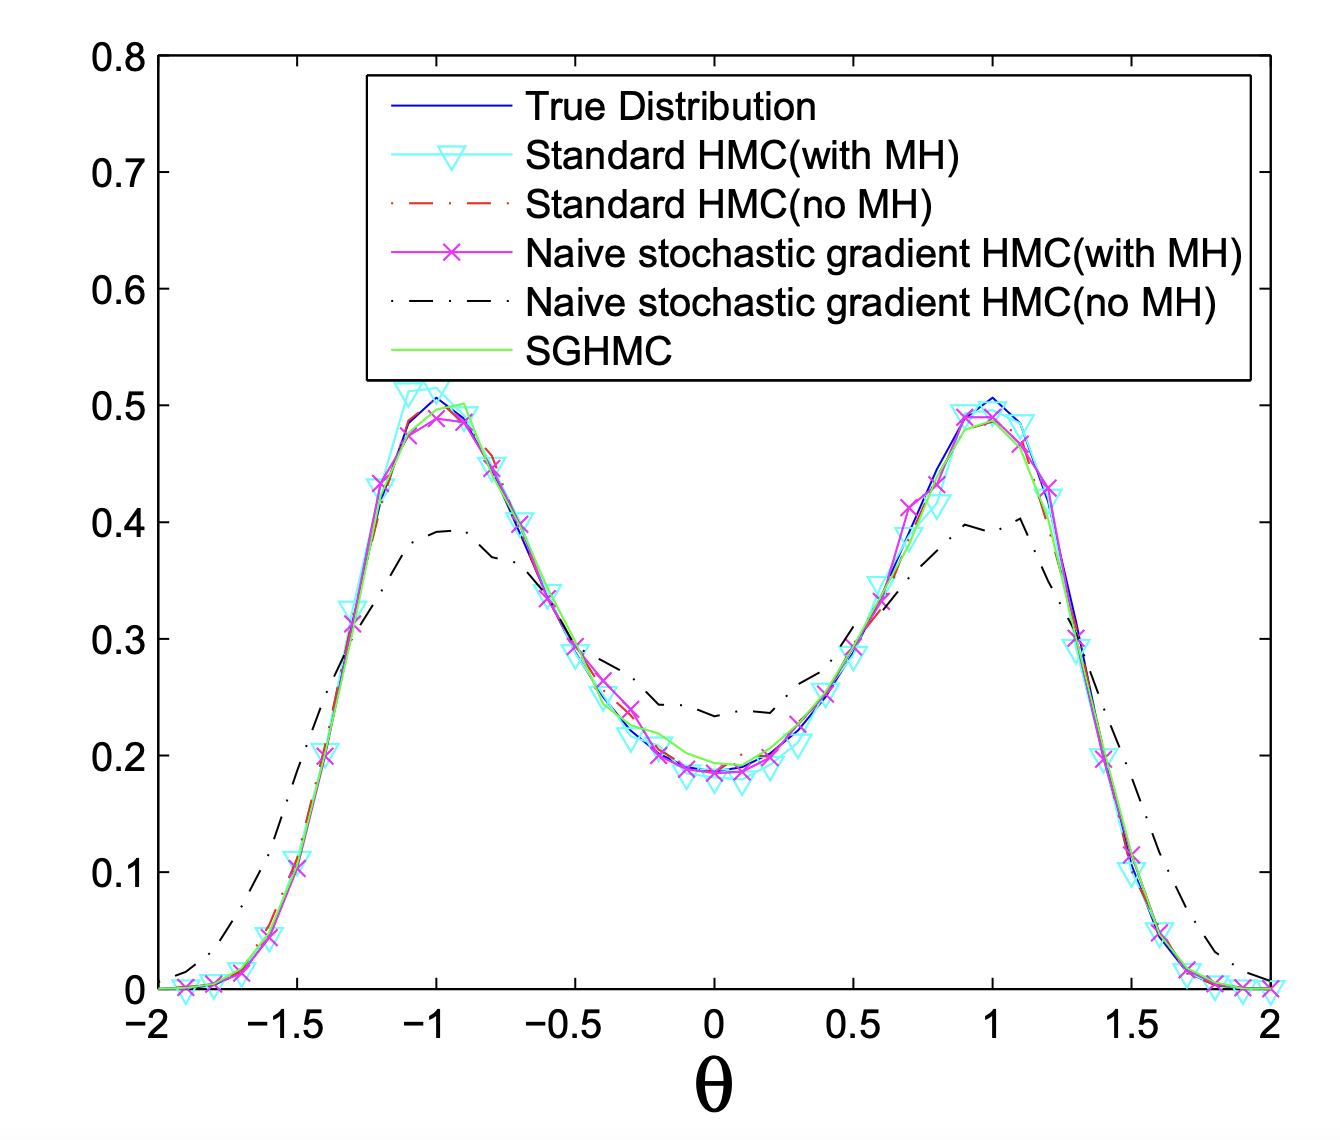
\includegraphics[width=100mm]{Images/reproduce2.png}
            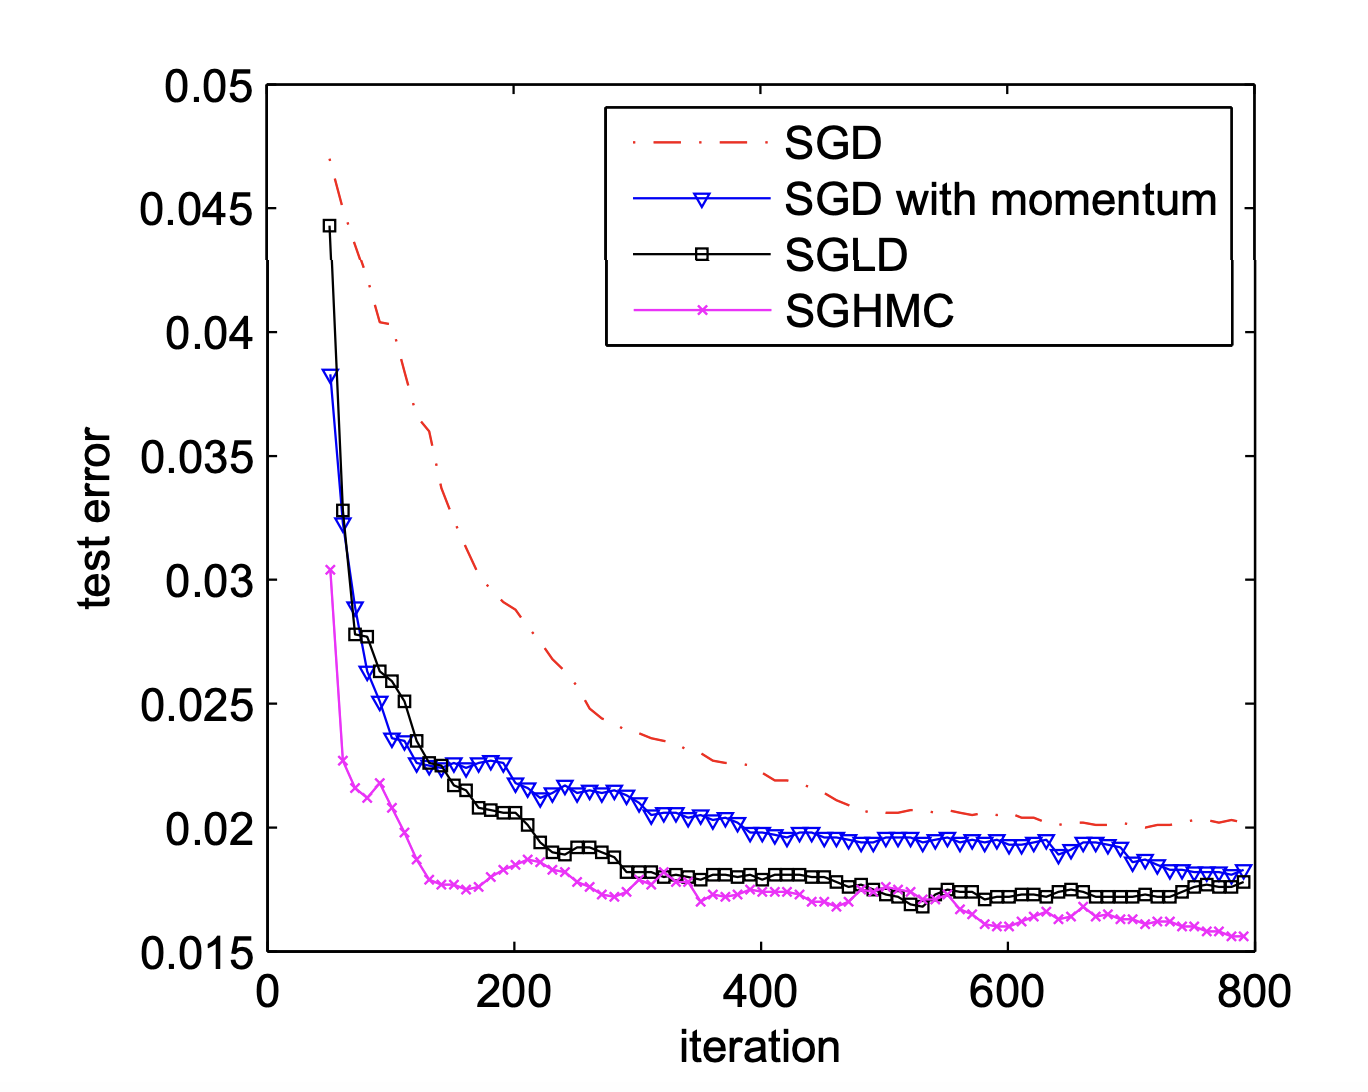
\includegraphics[width=100mm]{Images/reproduce3.png}
            \end{tikzfigure}

		We also extended the results of \cite{sghmc} in a number of ways:
		
	\begin{itemize}
    \item We extended the 'No U-Turn Sampler' (NUTS) from \cite{nuts} to work with SGHMC to produce our novel algorithm SGNUTS.
    \item Ran the Bayesian neural network (BNN) for classification experiment on a new dataset, namely, FashionMNIST \cite{fashion-mnist}.
    \item We demonstrated that our implementation of SGHMC can be used with Convolutional Neural Networks (CNNs) to classify CIFAR10 \cite{cifar10}.
    \item We implemented a scheme for estimating the gradient noise ($B$ in the literature and in what follows) and used this to increase the algorithm's sampling accuracy.
\end{itemize}
		
	}

    		\block{Implementation Details}{We implemented the following algorithms from scratch: HMC, SGHMC, SGLD , SGD, SGD with Nesterov momentum and SGNUTS. All of our implementations subclass Pyro's \texttt{MCMCKernel} and are designed to be used directly with Pyro \cite{pyro} — a universal probabilistic programming language (PPL) written in Python. Pyro comes with useful built in functions that transform probabilistic programs (PP) into potential functions that automatically handle gradient computations. The main caveat of stochastic gradient samplers and optimizers is that we require that the potential function has the form: $$\widetilde{U}(\theta) =  -\frac{|\mathcal{D}|}{|\widetilde{\mathcal{D}}|} \log p(\widetilde{\mathcal{D}} \: | \: \theta) - \log p (\theta)$$
Using our implementations we illustrate below how sampling algorithms differ from optimization algorithms; while sampling algorithms visit the full posterior $p(\theta \: | \: \mathcal{D})$ as they draw samples, optimization algorithms hone in on the MAP estimate $\text{argmax}_{\theta} \{ p(D \: | \: \theta) \cdot p(\theta) \}$. 
	\begin{tikzfigure}[{\bf Far left}: SGHMC (\texttt{batch\_size} $= 5, \eta = 0.01, \alpha=0.1$ \texttt{num\_steps}$=10$, \texttt{resample\_n} $=50$). {\bf Mid left:} SGLD (\texttt{batch\_size} $= 5, \eta = 0.1, \alpha=0.1$ \texttt{num\_steps}$=5$). {\bf Mid right:} SGD (\texttt{batch\_size} $= 5, \eta = 0.001$). {\bf Far right:} SGD with Nesterov momentum (\texttt{batch\_size} $= 5, \eta = 0.001, \alpha=0.1$)]
            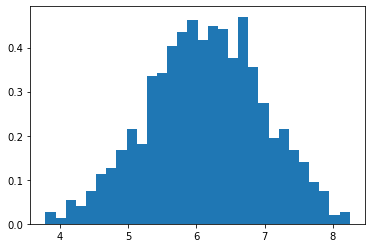
\includegraphics[width=75mm]{Images/SGHMC_demo.png}
            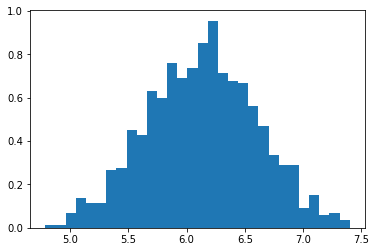
\includegraphics[width=75mm]{Images/SGLD_demo.png}
	    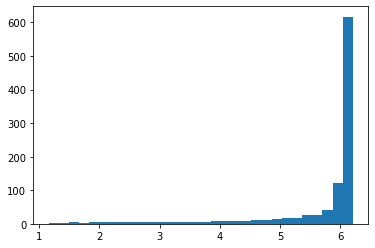
\includegraphics[width=75mm]{Images/SGD_demo.png}
            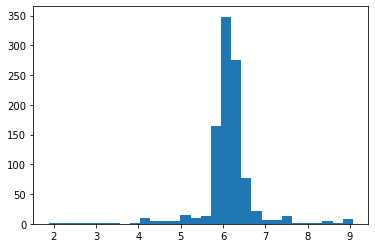
\includegraphics[width=75mm]{Images/SGDMOM_demo.png}
            \end{tikzfigure}
 }
		
\block{Simulated Examples}{
			Below we present our reproductions of the simulated scenarios in Section 4.1 of \cite{sghmc}. We implemented these toy examples in Python using the Matlab codes provided by the authors of the original paper \cite{simu_code}. We draw the following conclusions:
		\begin{itemize}
        \item Fig. 5(a) illustrates that the naive SGHMC fails to maintain the target distribution as its invariant distribution unless we add a costly MH correction step. Conversely, by adding friction, SGHMC maintains the target distribution as its invariant distribution, which validates the theoretical results in \cite{sghmc}.
        \item Fig. 5(b) shows that friction (green) keeps Hamiltonian dynamics much closer to the true Hamiltonian dynamics (blue) in a noisy system. Fig. 5(b) supports the results of Theorem 3.1 in \cite{sghmc}, that the sampled distribution tends to the uniform distribution over time, rather than the target distribution.
        \item Shown in Fig. 5(c): we see that for small step sizes SGLD \cite{sgld} has a high autocorrelation time while SGHMC has a very low autocorrelation time with even lower estimation error. This indicates the advantage of adopting SGHMC. Fig. 5(d) shows that SGLD performs worse in exploring the tails of the distribution when compared to SGHMC.
        \end{itemize} 
	\begin{tikzfigure}[{\bf (a)}: $\theta$ samples generated from $U(\theta) = -2\theta^2 + \theta^4$. {\bf (b):} 360 samples of $(\theta,r)$ generated from $U(\theta) = \frac{1}{2}\theta^2$ . {\bf (c):} Autocorrelation time versus mean absolute error of sample covariance for $U(\theta)=\frac{1}{2}\theta^T\Sigma^{-1}\theta$. {\bf (d):} First 50 samples of SGHMC and SGLD generated from $U(\theta)=\frac{1}{2}\theta^T\Sigma^{-1}\theta$]
	   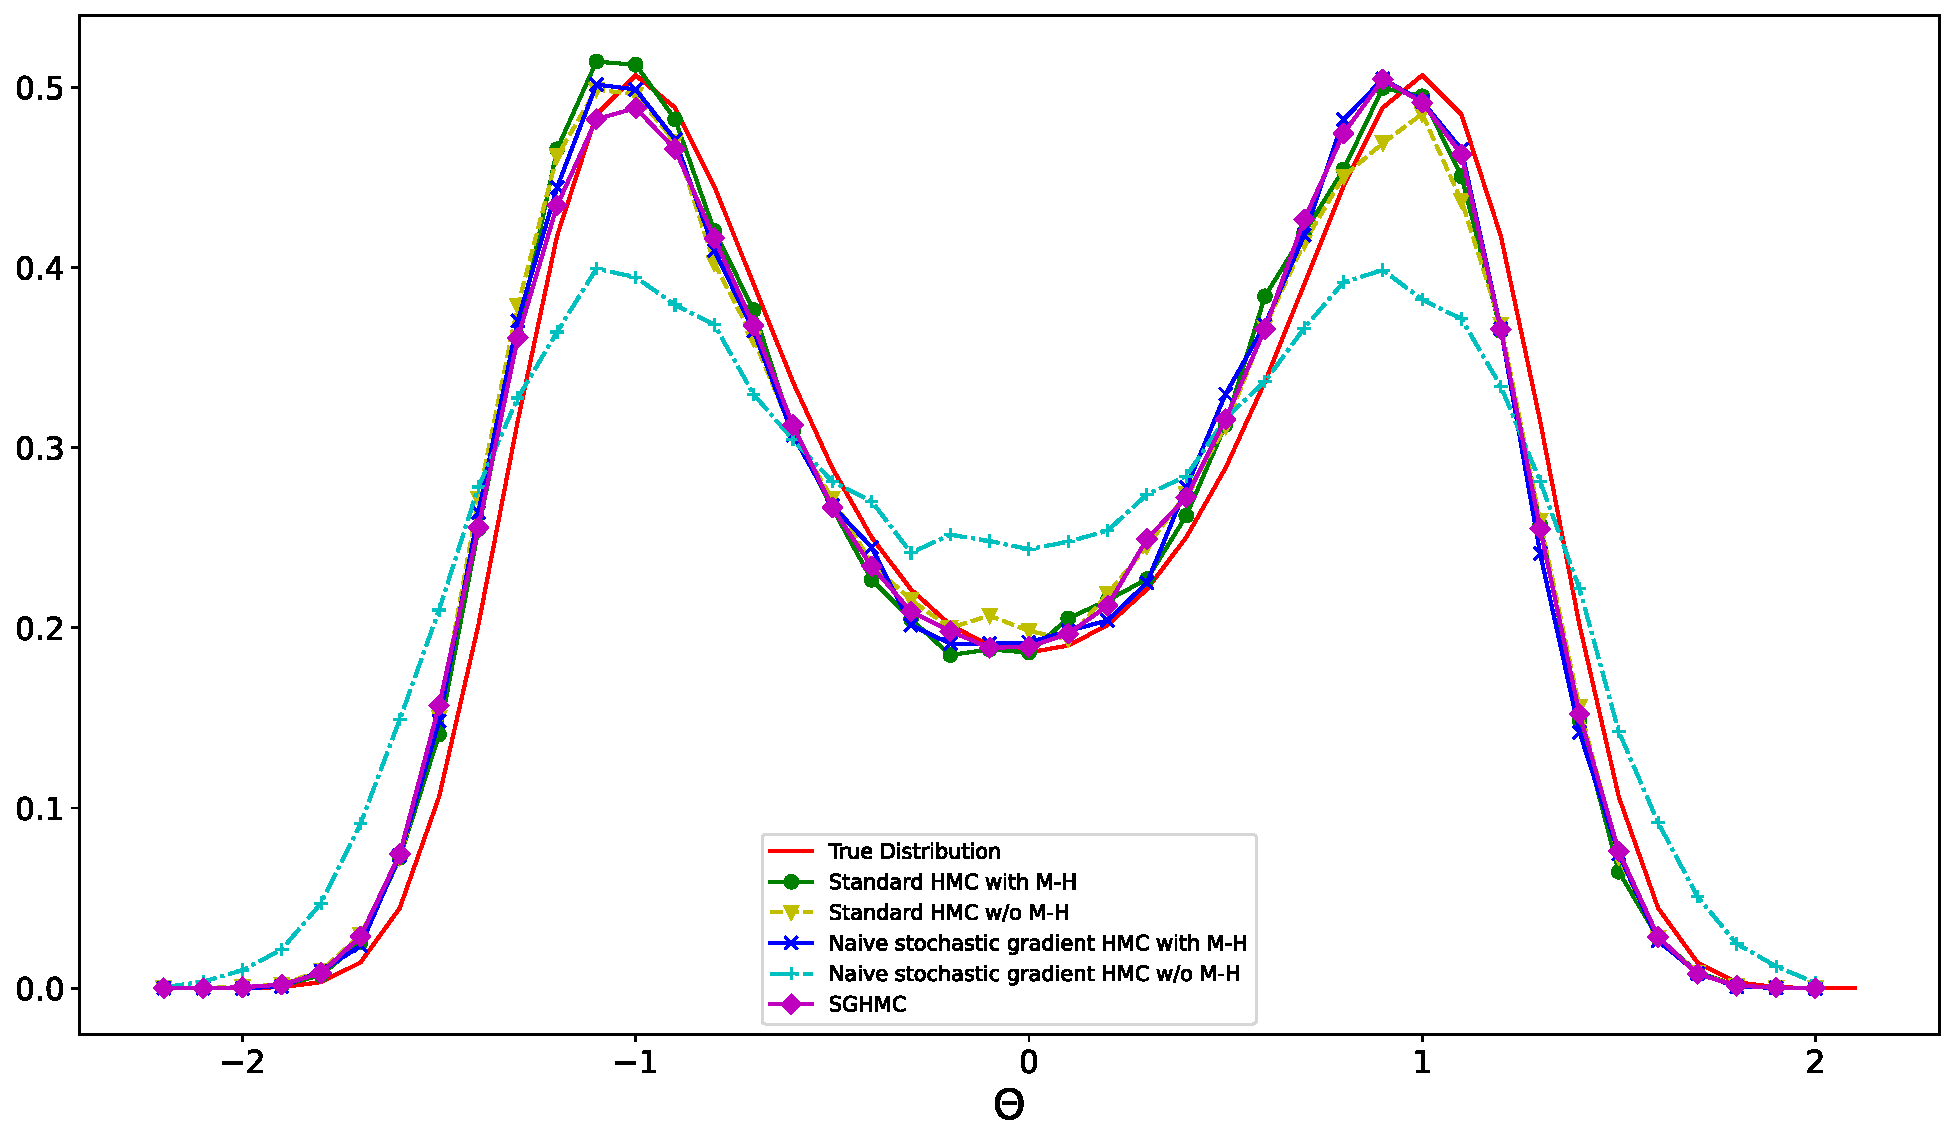
\includegraphics[width=120mm]{Images/fig1ax4.pdf}
            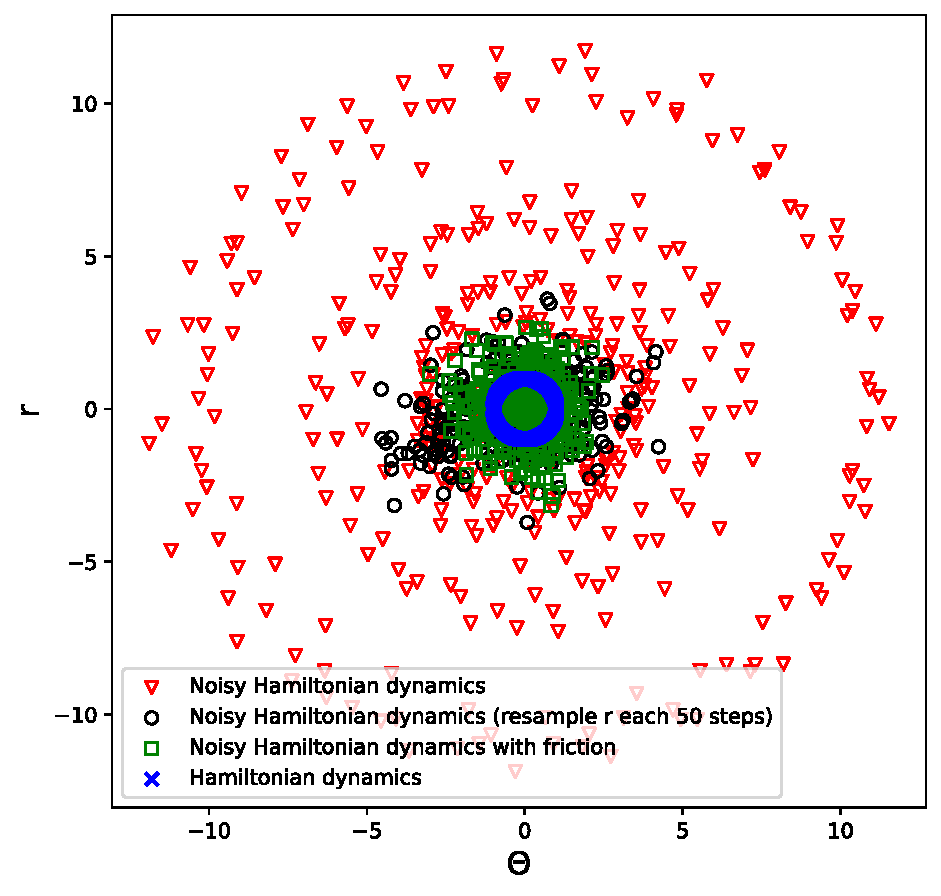
\includegraphics[width=75mm]{Images/fig2apt.pdf}
	    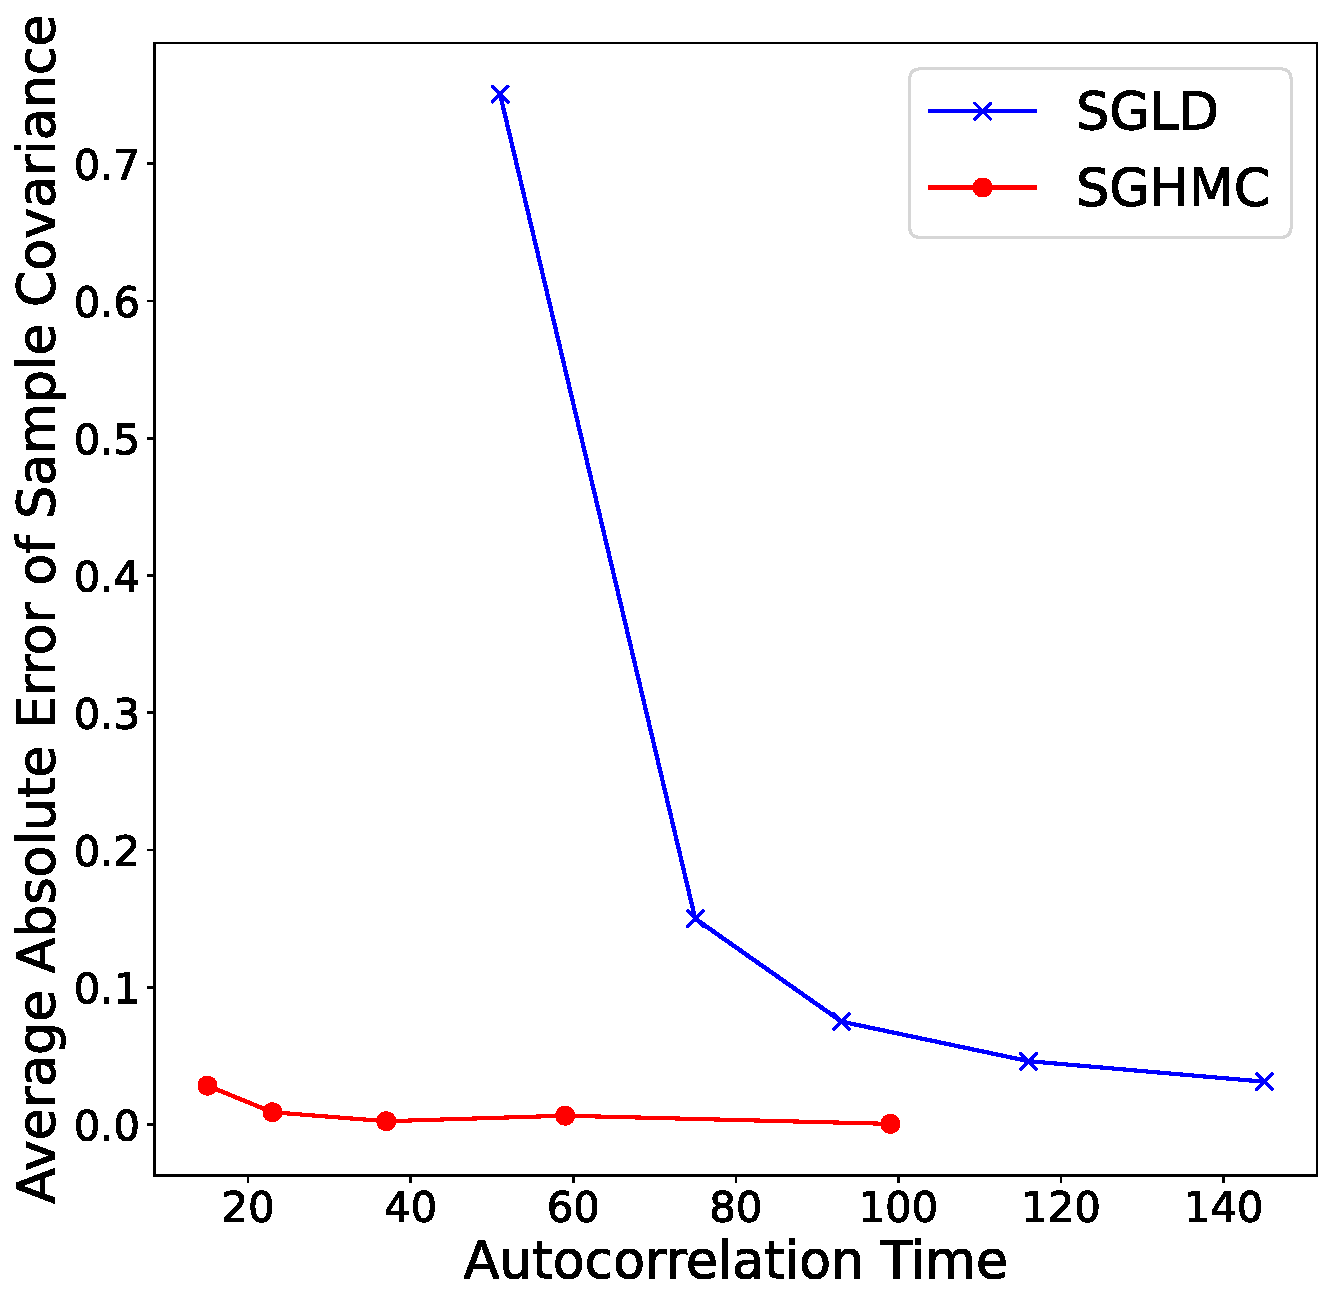
\includegraphics[width=75mm]{Images/fig3aerrt.pdf}
            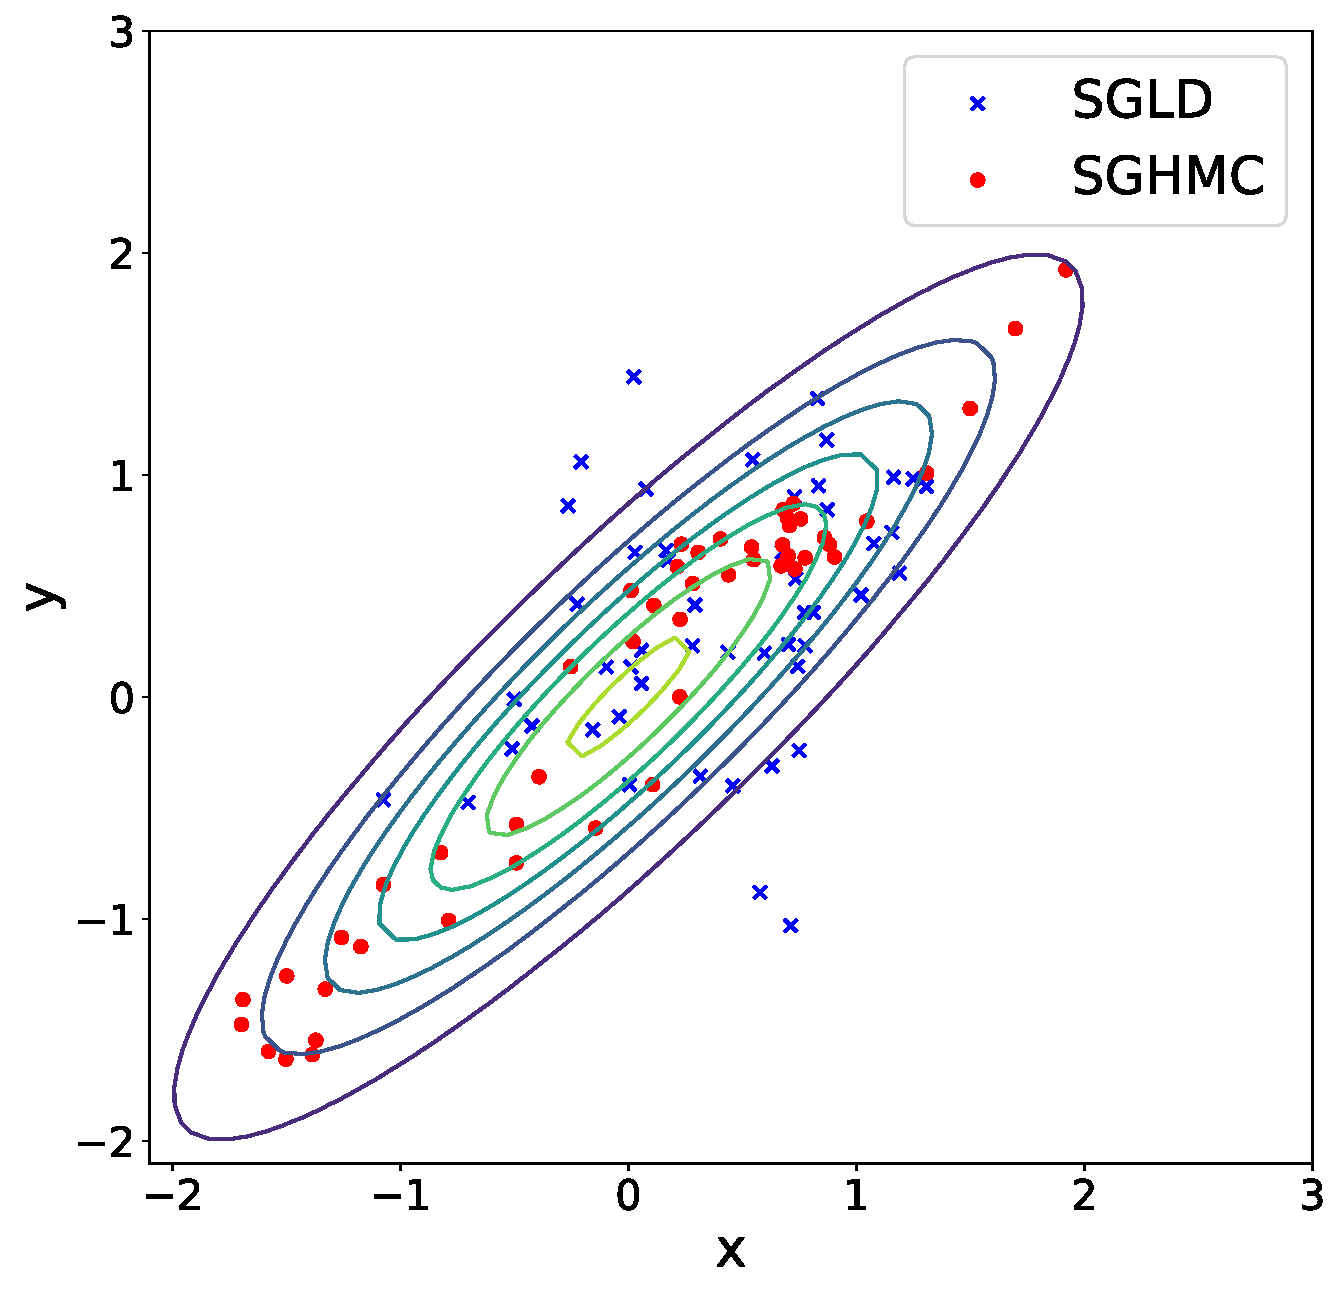
\includegraphics[width=75mm]{Images/fig3btraj.pdf}
            \end{tikzfigure} 		
	}
		

	\block{References}{
		\printbibliography[heading=none]
}
		
	\end{columns}
	



\end{document}